\documentclass{article}
\usepackage{booktabs}
\usepackage[a4paper, top=2cm, bottom=2cm, left=2.6cm, right=2.6cm]{geometry} % Keep only one geometry package
\usepackage[utf8]{inputenc}
\usepackage{amsmath}
\usepackage{eurosym}
\usepackage[T1]{fontenc}
\usepackage[french]{babel}
\usepackage{graphicx}
\usepackage{caption}
\usepackage{float}
\usepackage{multirow}
\usepackage{blindtext}
\usepackage{hyperref}
\usepackage{setspace} % Required for \onehalfspacing
\usepackage{subcaption}
\usepackage{longtable}

\begin{document}

\normalsize

\begin{titlepage}
\begin{center}

\includegraphics[width=0.7\textwidth]{images_titre/ensai_logo.png}\\[2.0 cm] 

\rule{\linewidth}{0.4mm} \\[0.4cm]
{\Large\bfseries Quelles circonstances sont associées à l’expression de signes cliniques respiratoires des porcs en croissance en élevages alternatifs?}\\[0.2cm]
\rule{\linewidth}{0.4mm}\\[3cm]

\begin{flushleft} \large
\emph{\underline{Étudiants:}}\\[0.2cm]
Antoni \textsc{Guàrdia Sanz} \\
Clément \textsc{Yvernault-Collet} \\
Marius \textsc{Vinclair}\\
Xavier \textsc{Braquaval}\\
\end{flushleft}

\begin{flushright} \large
\emph{\underline{Tutrice:}} \\[0.2cm]
Christelle \textsc{Fablet} \\[0.6cm]
\end{flushright}

\vfill
{\large \today}
\end{center}
\end{titlepage}

\newpage
\tableofcontents 
\newpage

\section{Introduction}
\subsection{Introduction du sujet}
\subsection{Description de la base de données}
\newpage
\section{Etude des variables respiratoires}
Dans cette section, on se propose d’analyser les relations entre les variables caractérisant la respiration des porcs, en particulier les fréquences d’éternuements et de toux en engraissement et post-sevrage, afin d’identifier les liens existants. L’objectif est de regrouper ces variables et de simplifier l’étude en réduisant leur complexité. Les analyses sont menées en omettant les variables manquantes.
\subsection{Présentation et caractérisation des variables respiratoires}
Dans cette partie, nous présentons et caractérisons les variables respiratoires mesurées chez les porcs. L'objectif est de mieux comprendre la répartition de ces données et d'identifier d'éventuelles particularités dans le comportement respiratoire des porcs.
%\begin{table}[h]
%    \centering
%    \begin{tabular}{lcccc}
%        \toprule
%        & Eter. PS & Eter. Eng & Toux PS & Toux ENG \\
%        \midrule
%        Min.   & 0.0000  & 0.0000  & 0.0000   & 0.000  \\
%        Q1 & 0.5401  & 0.0000  & 0.0000   & 0.000  \\
%        Medianne  & 3.1429  & 0.7587  & 0.7767   & 1.524  \\
%        Moyenne    & 9.0345  & 2.1773  & 6.2761   & 7.119  \\
%        Q3 & 10.0000 & 2.9241  & 5.5303   & 8.472  \\
%        Max.    & 88.8889 & 16.1290 & 137.0370 & 70.000 \\
%        NA's    & 1       & 4       & 1        & 4      \\
%        \bottomrule
%    \end{tabular}
%    \caption{Caractérisation des variables respiratoires}\label{tab:summary_stats}
%\end{table}

\begin{figure}[h]
    \centering
    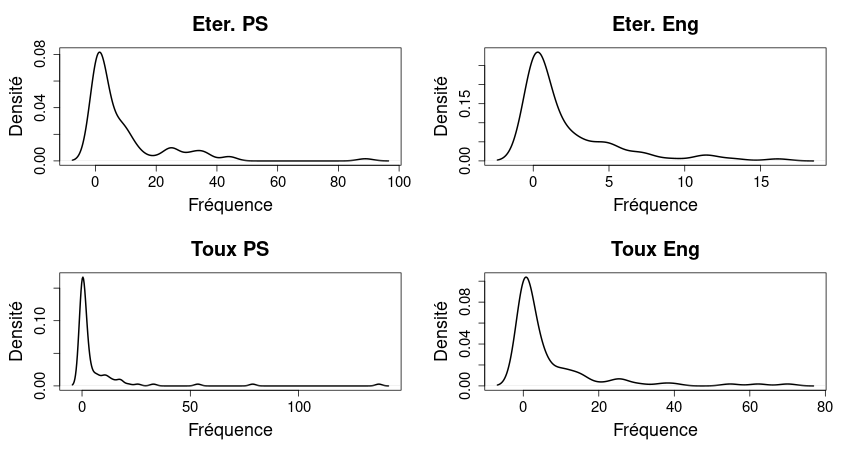
\includegraphics[width=\textwidth]{img_var_resp/dens_var_resp.png}
    \caption{Densité des variables respiratoires (BP\protect\footnotemark\ \text{: }nrd0\protect\footnotemark)}\label{fig:dens_resp}
\end{figure}

\addtocounter{footnote}{-1}
\footnotetext[\thefootnote]{Bande passante.} 
\addtocounter{footnote}{1}
\footnotetext[\thefootnote]{La méthode \texttt{nrd0} fait référence à la largeur de bande de référence normale.}

Notons que dans (\ref{fig:dens_resp}) les quatre variables respiratoires présentent une forte concentration de la densité autour de 0, ce qui reflète un bon état respiratoire global chez les porcs étudiés. Cependant, certains élevages montrent des exceptions où cette tendance générale n'est pas observée.

\begin{figure}[h]
    \centering
    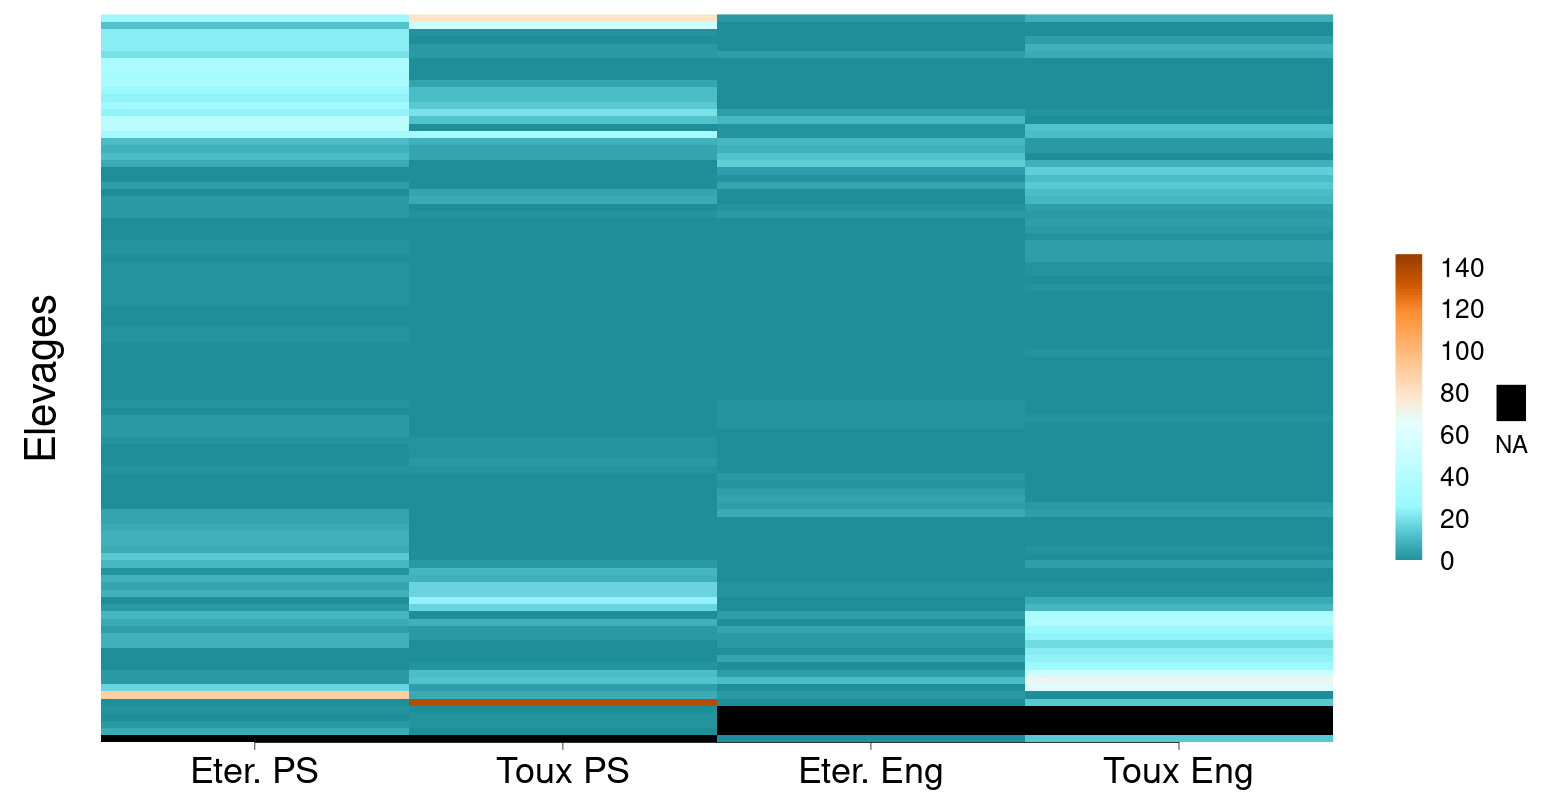
\includegraphics[width=0.9\textwidth]{img_var_resp/rep_var_resp.png}
    \caption{Visualisation des variables respiratoires par élevages}\label{fig:rep_resp}
\end{figure}
\newpage
Dans (\ref{fig:rep_resp}), nous constatons une fois de plus que la majorité des individus présentent des valeurs faibles pour l'ensemble des variables respiratoires. Nous relevons également la présence de cinq individus avec des valeurs manquantes. Il apparaît que ces valeurs manquantes concernent soit les variables issues de l'engraissement, soit celles du post-sevrage. Cette observation est cohérente avec le protocole de l'étude, qui prévoyait la mesure simultanée des éternuements et des toux.
Des légères corrélations entre la toux et les éternuements sont également observées au sein d'un même lot.
\subsection{Exploration des relations entre les variables respiratoires}
L'objectif de cette section est d'analyser la force des liens entre les variables respiratoires, afin de déterminer si une régression linéaire pourrait être pertinente pour réduire le nombre de variables à considérer dans les étapes suivantes. De plus, cette exploration permet d'évaluer la pertinence de l'Analyse en Composantes Principales (ACP) pour la réduction de dimensions, afin de juger de son adéquation avec nos données.

\subsubsection{Relations linéaires entre les variables respiratoires}
Examinons les corrélations ainsi que la répartition des élevages selon les variables respiratoires.
\begin{figure}[htbp]
    \centering
    \begin{subfigure}[b]{0.49\textwidth}
        \centering
        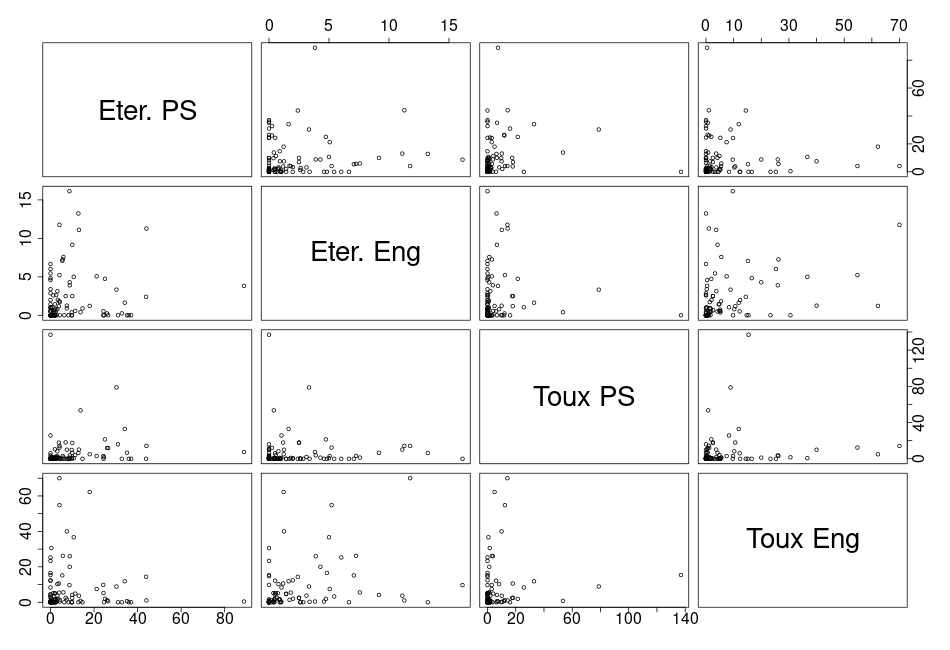
\includegraphics[width=\textwidth]{img_var_resp/points_corr_lin.png}
        \caption{Répartition des élevages}\label{fig:disp_lin}
    \end{subfigure}
    \hspace{0.1cm}
    \begin{subfigure}[b]{0.49\textwidth}
        \centering
        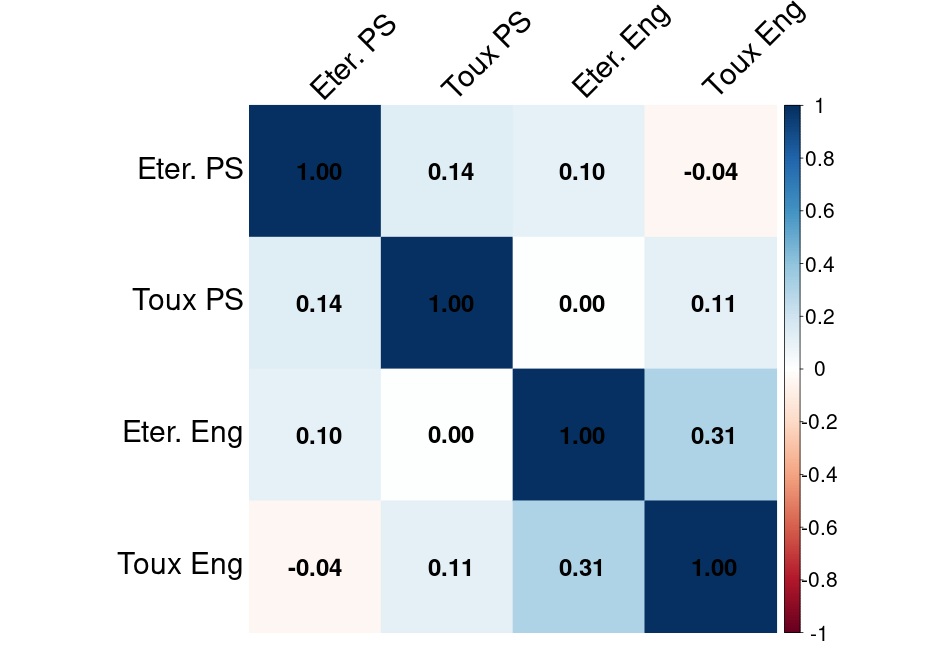
\includegraphics[width=\textwidth]{img_var_resp/corrplot_corr_lin.png}
        \caption{Matrice des correlations}\label{fig:corr_mat_lin}
    \end{subfigure}
    \caption{Illustration étude linéaire}\label{fig:etu_lin}
\end{figure}

Dans la figure (\ref{fig:etu_lin}), aucune relation linéaire forte n’apparaît entre les différentes variables. Ce constat est particulièrement évident dans la figure (\ref{fig:disp_lin}), où les nuages de points ne présentent pas la structure triangulaire typique d’une dispersion linéaire.
Cependant, la matrice de corrélation (\ref{fig:corr_mat_lin}) met en évidence des faibles corrélations entre la plupart des variables, à l’exception notable des éternuements en engraissement et des toux en post-sevrage. On observe en effet une corrélation marquée entre les toux et les éternuements, qui appartiennent au même groupe (soit engraissement, soit post-sevrage), cette corrélation étant particulièrement prononcée chez les porcs en engraissement.
Le test de Pearson confirme ces observations (Cf.\text{ }\ref{annexe:pearson}): la seule corrélation statistiquement significative concerne les variables toux et éternuements en engraissement.

Les analyses graphiques et le test de Pearson révèlent une absence de relations linéaires globales entre les variables, à l'exception de la corrélation entre toux et éternuements en engraissement. Par conséquent, l'ACP, qui repose sur des hypothèses de linéarité, ne semble pas être la méthode d'analyse la mieux adaptée à ce jeu de données.


\subsubsection{Relations logarithmiques entre les variables respiratoires}
Nous appliquons la transformation $x \longmapsto \ln(x \cdot \hat{{\sigma_x}} + 1)$\text{ }\footnote{Nous utilisons la transformation \( x \longmapsto \ln(x \cdot \hat{{\sigma_x}} + 1) \) plutôt que \( x \longmapsto \ln(x) \cdot \hat{{\sigma_x}} \) afin de tenir compte de la présence de zéros dans nos données, tout en conservant une fonction bien définie. Le facteur \( \hat{{\sigma_x}}  \) (écart-type) est ajouté pour normaliser les données, en atténuant l'effet des différences de dispersion entre les variables, ce qui permet de stabiliser la variance et de rendre les données plus comparables.}
Examinons maintenant les corrélations ainsi que la répartition des élevages selon les nouvelles données.

\newpage

\begin{figure}[htbp]
    \centering
    \begin{subfigure}[b]{0.49\textwidth}
        \centering
        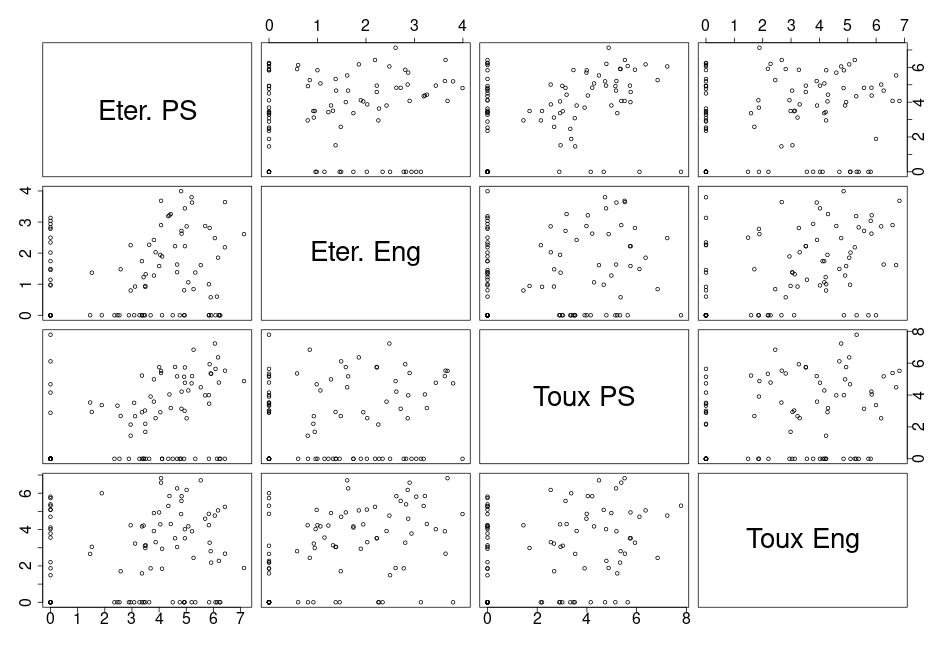
\includegraphics[width=\textwidth]{img_var_resp/points_corr_log.png}
        \caption{Répartition des élevages}\label{fig:disp_log}
    \end{subfigure}
    \hspace{0.1cm}
    \begin{subfigure}[b]{0.49\textwidth}
        \centering
        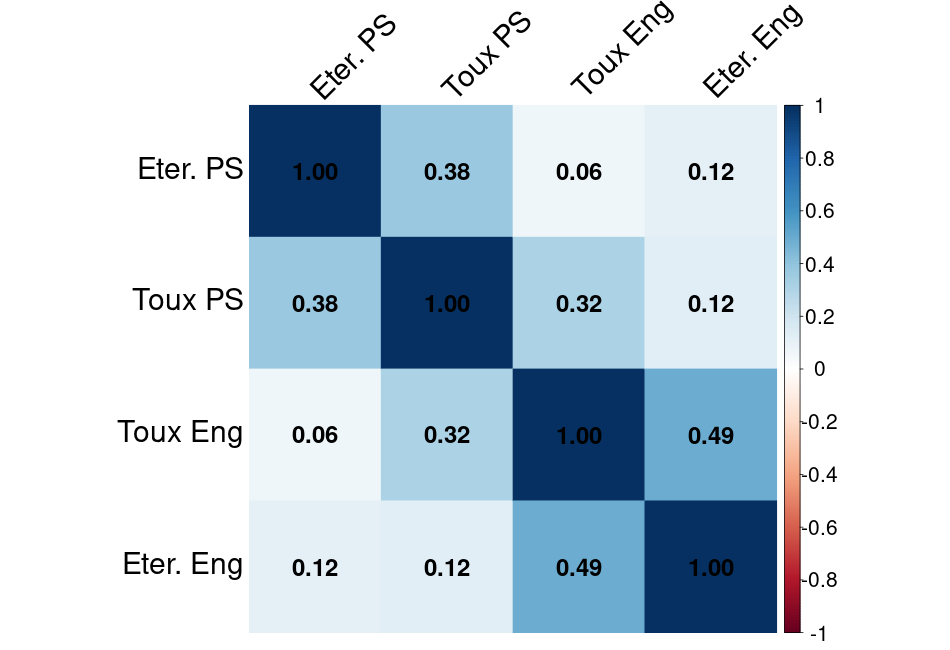
\includegraphics[width=\textwidth]{img_var_resp/corrplot_corr_log.png}
        \caption{Matrice des correlations}\label{fig:corr_mat_log}
    \end{subfigure}
    \caption{Illustration étude logarithmique}\label{fig:etu_log}
\end{figure}

Cette fois-ci, nous observons qu'il pourrait exister une relation linéaire entre les logarithmes des variables respiratoires (\ref{fig:disp_log}). Notamment, cette relation linéaire est particulièrement visible pour les variables toux post-sevrage et éternuements post-sevrage.
Observons également que dans (\ref{fig:disp_log}), trois groupes de points se distinguent clairement. En considérant les deux variables précédentes, ces groupes peuvent être interprétés comme suit:
\vspace{0.25cm}
\begin{itemize}
\item Absence d’éternuements en post-sevrage
\item Absence de toux en post-sevrage
\item Présence simultanée de toux et d’éternuements en post-sevrage
\end{itemize}
\vspace{0.25cm}
C’est dans ce dernier groupe que l'on observe une relation plus ou moins linéaire entre ces deux variables.
Dans (\ref{fig:corr_mat_log}), cette relation est à nouveau perceptible entre les variables d'engraissement et celles du post-sevrage. De plus, une corrélation relativement forte est mise en évidence entre la toux en post-sevrage et l’engraissement.
Ces observations graphiques sont confirmées par les tests de Pearson (\ref{annexe:pearson_log}).

Cependant, il paraît difficile d’expliquer une variable à partir des trois autres, même au sein du sous-groupe d’élevages qui semble le mieux s’adapter à un modèle linéaire, en raison de la forte amplitude du bruit\footnote{En (\ref{annexe:reg_lin_log}), une régression linéaire est détaillée afin de modéliser le logarithme des toux en post-sevrage. Les résultats obtenus montrent toutefois une capacité explicative limitée du modèle, avec un coefficient de détermination de  $R^2=0.4$}. De plus, les autres sous-groupes d’élevages ne semblent pas non plus adaptés à ce type d’approche.

\subsection{Simplification des variables respiratoires}
À cette étape, nous proposons de regrouper les élevages en différentes classes afin de réduire le nombre de variables explicatives en une seule. Pour ce faire, nous utilisons la méthode de réduction de dimension UMAP\footnote{\textit{Uniform Manifold Approximation and Projection} en anglais. C’est une technique de réduction de dimension qui permet de représenter des données complexes dans un espace de dimension inférieure tout en conservant au mieux leur structure.}, qui s’adapte bien aux structures non linéaires de nos variables. Ensuite, nous appliquons une classification hiérarchique ascendante afin de constituer des groupes d’élevages, qui seront ensuite analysés et interprétés.
\subsubsection{Réduction des dimensions}
On fait le choix arbitraire de réduire les variables en deux dimensions avec UMAP et on apliqque la classification hiérarchique ascendante (CHA) on obtient alors les résultat suivant:

\newpage

\section{Imputation des variables manquantes}

\newpage
\appendix

\section{Annexe: compléments de l'analyse sur les variables respiratoires}
\subsection{Test de pearson sur les corrélations des variables réspiratoires}\label{annexe:pearson}

\begin{table}[ht]
    \centering
    \begin{tabular}{llccc}
    \toprule
    \textbf{Variable 1} & \textbf{Variable 2} & \textbf{Coefficient de corrélation} & \textbf{p-valeur} & \textbf{Significatif} \\
    \midrule
    Eter. PS & Eter. Eng & 0.104 & 0.317 & Non \\
    Eter. PS & Toux PS & 0.135 & 0.191 & Non \\
    Eter. PS & Toux Eng & -0.041 & 0.696 & Non \\
    Eter. Eng & Toux PS & 0.003 & 0.979 & Non \\
    Eter. Eng & Toux Eng & 0.305 & 0.003 & Oui \\
    Toux PS & Toux Eng & 0.114 & 0.273 & Non \\
    \bottomrule
    \end{tabular}
    \caption{Résultats des tests de corrélation de Pearson entre les variables respiratoires.}\label{tab:correlation_results}
\end{table}
Constatons que la seule corrélation significative est celle des variables de toux et éternouments en engraissement. 
\subsection{Test de pearson sur les corrélations du logarithme des variables réspiratoires}\label{annexe:pearson_log}
\begin{table}[ht]
    \centering
    \begin{tabular}{llccc}
    \toprule
    \textbf{Variable 1} & \textbf{Variable 2} & \textbf{Coefficient de corrélation} & \textbf{p-valeur} & \textbf{Significatif} \\
    \midrule
    Eter. PS & Eter. Eng & 0.119 & 0.251 & Non \\
    Eter. PS & Toux PS & 0.377 & 0.000 & Oui \\
    Eter. PS & Toux Eng & 0.061 & 0.557 & Non \\
    Eter. Eng & Toux PS & 0.122 & 0.240 & Non \\
    Eter. Eng & Toux Eng & 0.491 & 0.000 & Oui \\
    Toux PS & Toux Eng & 0.315 & 0.002 & Oui \\
    \bottomrule
    \end{tabular}
    \caption{Résultats des tests de corrélation de Pearson entre les variables respiratoires.}\label{tab:correlation_log_results}
\end{table}
TODO


\subsection{Résultats régression linéaire entre les variables respiratoires et leur logarithme}\label{annexe:reg_lin_log}
TODO GLS with log transform 

\subsection{Résultats classification}

\begin{table}[ht]
    \centering
    \begin{tabular}{lcccc}
        \toprule
        \textbf{Variable} & \textbf{v.test} & \textbf{$\bar{x}$ (var)} & \textbf{$\bar{x}$ (total)} & \textbf{$\sigma_x$ (var)} \\
        \midrule
        ENG\_Eter\_freq & 6.73 & 5.55 & 2.20 & 3.94 \\
        ENG\_Tx\_freq  & 4.67 & 16.31 & 7.04 & 19.46 \\
        \midrule
        \textbf{p.value} & 1.75e-11 & & & \\
        \bottomrule
    \end{tabular}
    \caption{ENG\_malade\_var}
\end{table}
    
    % Table for PS_malade
\begin{table}[ht]
    \centering
        \begin{tabular}{lcccc}
        \toprule
        \textbf{Variable} & \textbf{v.test} & \textbf{$\bar{x}$ (var)} & \textbf{$\bar{x}$ (total)} & \textbf{$\sigma_x$ (var)} \\
        \midrule
        PS\_Eter\_freq & 6.35 & 26.39 & 9.27 & 18.71 \\
        PS\_Tx\_freq  & 4.58 & 21.98 & 6.50 & 32.00 \\
        \midrule
        \textbf{p.value} & 2.21e-10 & & & \\
        \bottomrule
    \end{tabular}
    \caption{PS\_malade\_var}
\end{table}
    
    % Table for Sain
\begin{table}[ht]
    \centering
    \begin{tabular}{lcccc}
        \toprule
        \textbf{Variable} & \textbf{v.test} & \textbf{$\bar{x}$ (var)} & \textbf{$\bar{x}$ (total)} & \textbf{$\sigma_x$ (var)} \\
        \midrule
        PS\_Tx\_freq    & -2.66 & 1.34 & 6.50 & 2.55 \\
        ENG\_Tx\_freq   & -3.53 & 1.92 & 7.04 & 3.15 \\
        PS\_Eter\_freq  & -4.19 & 2.78 & 9.27 & 3.59 \\
        ENG\_Eter\_freq & -4.92 & 0.41 & 2.20 & 0.53 \\
        \midrule
        \textbf{p.value} & 7.75e-03 & & & \\
        \bottomrule
    \end{tabular}
    \caption{Sain\_var}
\end{table}

\end{document}
